\chapter{Implementation}

\begin{comment}
Chapter 4: Implementation
The implementation details should be confined to the important, difficult or interesting aspects. Large chunks of code should be avoided, and diagrams and tables should be used to present details clearly.
\end{comment}

\plan{Limited to programming languages only}

\begin{comment}
Statement Management 
Upload
NamedEntityResolution
Suggestions ........................ 19

Prediction
MarkovChain
WeightedArithmeticMean
FiveModelSystem
Confidence

Security Considerations
AccountHijacking
PasswordSecurity
Database Security
Other
\end{comment}

This section is focused on particularly interesting or troublesome parts of implementing the design outlined in \ref{cha:design} and any usage of external libraries. As it was decided the project would be a web application\todo{Should probably mention this in design} the user interface was written in HTML \& CSS, with the interactive elements such as the graphs in JavaScript. PHP was chosen as the server side language used to process the user and the database was implemented using MySQL.

PHP was selected as the server side language because the author had extensive experience in the language, it's original intended use was web development and it is well supported. It's intention of web development means it's well coupled with HTML and provides many libraries to handle it, giving the language a significant advantage over languages such as Python and Java which can be adapted for web use. A key disadvantage of PHP is that is it weak typed which lead to some issues during development where objects of the wrong type were passed into functions. This disadvantage was considered and it was decided the advantages outweighed the disadvantages.

The project uses a PHP Framework, written by the author \todo{This doesn't make sense} called pegFramework. Using a framework has several key advantages over writing the whole system.

Frameworks:
Provide standardised code and file organisation - pegFramework has a well defined code structure, code is organised in a predefined way and split into modules
MVC - Model View Controller - using the MVC pattern with a framework ensures models (data structures), views (page contnet) and controllers are separate, improving cohesiveness and decreasing coupling.
Utilities and libraries - frameworks handle all the standard web design code, including routing, security, controllers, rendering the template and caching.

MySQL was selected as the database language because it's well supported by PHP and because it provides Natural Language Searching out of the box, which supports free-text queries and can calculate the relevance of a record in the database to a search term. This is used to power the suggestions section of the website and for user entered searches.

Server Side Libraries:

Twig - a template engine that takes collections of PHP objects and following a provided .html template build the output sent to the browser. In addition it provides caching of the generated templates and output, leading to significant speed increases for the end user.

Propel - an object relational mapping (ORM) library for PHP. Propel takes a database schema defined in XML and generates PHP objects that represent the schema which can be saved to and loaded from the database.

Less - CSS pre-processor that extends CSS, adding additional features and inheritance. `.less` files compile to `.css`

Front End

Bootstrap - framework for CSS development that provides grid and stuff

jQuery - javascript development framework that abstracts differences in browser behaviour and provides shorthands to common tasks such as ajax requests

Pines Nofity - alerts

Chosen - javascript libray to make dropdown boxes better

Highcharts - charting library for the UI

\section{Statement Management}

\subsection{Upload}
OFX is an XML like format called SGML. PHP has inbuilt libraries for parsing XML called SimpleXML simplexml\_load\_string loads an XML file from a string. To parse the OFX, PHP attempts to parse it as an XML file and captures any exceptions. If exeptions are found it attempts to convert the SGML XML so it can be pased by PHP as per 

%http://stackoverflow.com/questions/15735330/how-to-parse-a-ofx-version-1-0-2-file-in-php and http://www.hanselman.com/blog/PostprocessingAutoClosedSGMLTagsWithTheSGMLReader.aspx

\todo{Comparison of SGML and XML}

For each line of the SGML it trims whitespace including (x,y,z), converts the charset ot UTF-8 so it's valid in PHP and if no closing tag is found, appends a closing tag

\lstset{style=phpcolor}
\begin{lstlisting}
foreach(preg_split("/((\r?\n)|(\r\n?))/", $this->OFXContent) as $line){
        		
        	// Trim whitespace
        	$line = trim($line);
        	if ($line === '') continue;
        
        	// Convert charset to UTF-8
        	$line = iconv($charset, 'UTF-8', $line);
        	if (substr($line, -1, 1) !== '>') {
        		list($tag) = explode('>', $line, 2);
        		$line .= '</' . substr($tag, 1) . '>';
        	}
        	$buffer .= $line ."\n";
}
\end{lstlisting}

Having parsed the SGML into objects it can just be navigated following the specification and converted to arrays of information for each transaction, refered to as movements. These movements look like XYZ; and can then be convered into the Transaction objects most of the fields are handled automatically but dates need to be handled specifically.

QIF is handled in a different manor as there are no native libraries to parse it's format. As shown in section X the file consists of movements, marked with \^'s and each field related to that movement is prefixed with a letter explaining what it's type.

D	Date
T	Amount
C	Cleared status
P	Payee
M	Memo
^	End of entry

Like the SGML the application loops though all the lines found in the file, switching on the prefix and sorting the information into the appropriate pieces of an array.

\lstset{style=phpcolor}
\begin{lstlisting}

// QIF line identifier
$id = substr($line, 0, 1);

// Rest of the line
$content = trim(substr($line, 1, strlen($line)));

switch ($id) {
	// End of entry
	case '^':
		// Completed transaction append to our list and reset
		$this->movements[] = $newMovement;
		$newMovement = array();
		break;
		
	// Amount
	case 'T':
		$newMovement["value"] = floatval(preg_replace("/[^0-9.-]/", "", $content));
		break;
		
	// Date
	case 'D':
		$newMovement["date"] = $content;
		break;
		
	// etc ...
\end{lstlisting}

As outlined in section \ref{subsection:upload} the conversion from array to Transaction is slightly more involved, this due to unknown date format. To implement this in PHP, all movements are tested against two regular expressions, representing the formats of the dates, visualised as graphs in Fig. \ref{regex-dmy} and \ref{regex-mdy}.

\begin{lstlisting}
$dmy = true;
$mdy = true;
foreach($this->getMovements() as $movement)
	if(!preg_match('#(0[1-9]|[12][0-9]|3[01])[-/](0[1-9]|1[012])[-/](19|20|21)?\d\d#', $date))
		$dmy = false;
	
	if(!preg_match('#(0[1-9]|1[012])[-/](0[1-9]|[12][0-9]|3[01])[-/](19|20|21)?\d\d#', $date))
		$mdy = false;
...

if($dmy && $mdy || !$dmy && !$mdy)
	// ... prompt the user
else
    // ... continue to parse the file in the detected format
\end{lstlisting}

\begin{figure}[h]
    \centering
    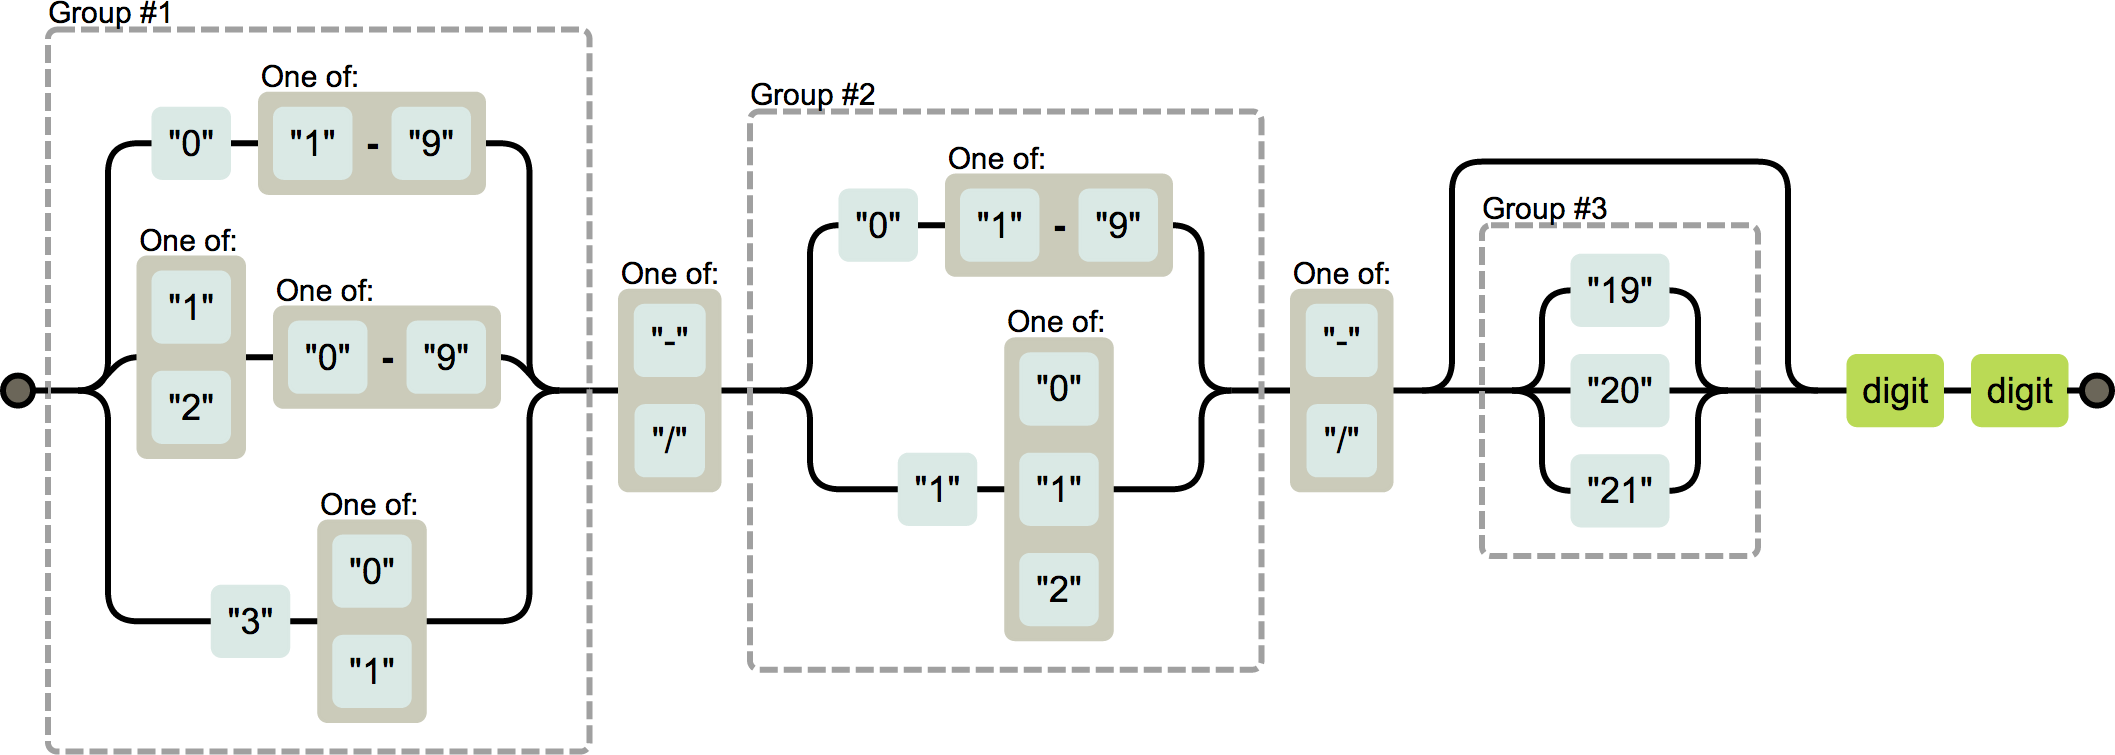
\includegraphics[width=0.70\textwidth]{implementation/regex-dmy}
    \caption{Regular expression used to match the date format d-m-Y}
    \label{fig:regex-dmy}
\end{figure}

\begin{figure}[h]
    \centering
    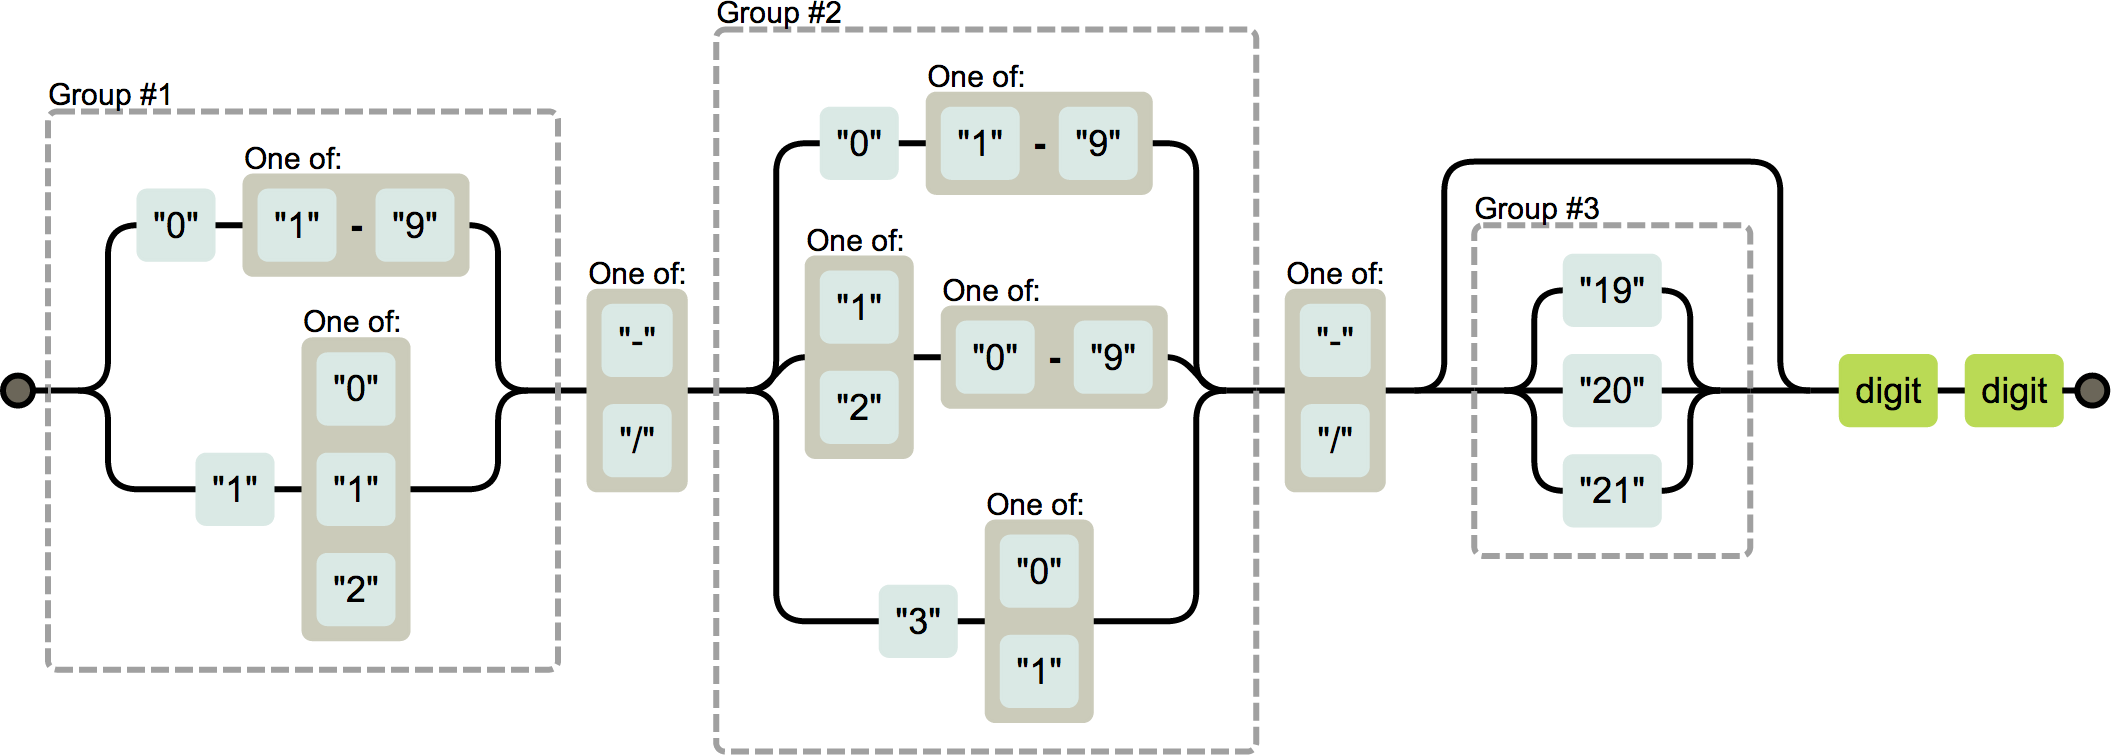
\includegraphics[width=0.70\textwidth]{implementation/regex-mdy}
    \caption{Regular expression used to match the date format m-d-Y}
    \label{fig:regex-mdy}
\end{figure}

\section{Trans}

\section{Prediction}
\plan{All the steps that were needed for the prediction}

\subsection{Named Entity Resolution}
\plan{Use of MySQL to find similar, how that works, alternatives}

\subsection{Suggestions}
\label{section:suggestion-implementation}
\plan{How it uses the above, how the whole user/global thing works}

\subsection{Markov Chain}
\plan{Why I chose first order markov chains, alternatives to that etc...}

\subsection{Weighted Averages}
\plan{How does that work, why is it good?}

\subsection{5 Model System}
\plan{How was is a model chosen for the user?}
